\begin{frame}{$"n"$ momentum vs IM of $\pi^+ \pi^-$}
  \tminipageTwo{
    \begin{figure}
      Data\\
      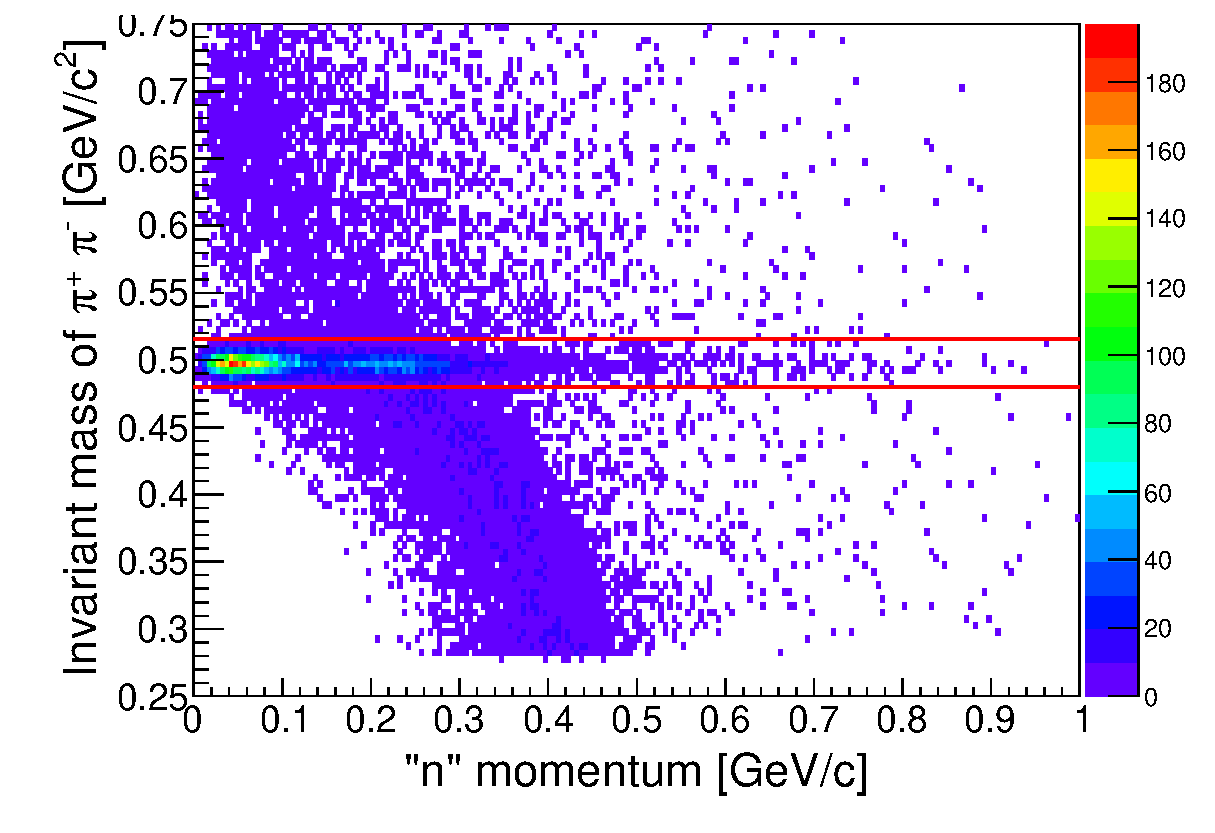
\includegraphics[width=5cm]{../pic/Run78/KN_ana/mmN_mom_IM_pipi_data.eps}
    \end{figure}
  }{
    \begin{figure}
      BG sum\\
      \includegraphics[width=5cm]{../pic/Run78/KN_ana/mmN_mom_IM_pipi_BG.eps}
    \end{figure}
  }

  \tminipageTwo{
    \begin{figure}
      \tiny
      \centering
      $d(K^-, n)"\pi^{\pm}\Sigma^{\mp}"$イベントでは$K^0$は3$\sigma$で除去\\
      \vspace{3mm}
      $d(K^-, n)"\pi^{\mp}\Sigma^{\pm}"$では$\pi^+ \pi^-$不変質量の\\低いところに位置する。\\
      $K^-d\rightarrow "n" \pi^{\mp} \Sigma^{\pm}$では$\pi^+ \pi^-$不変質量の\\高いところに位置する。\\
    \end{figure}
  }{
    \tminipageTwo{
      \begin{figure}
        \tiny
        $d(K^-, n) \pi^- \Sigma^+$\\
        \includegraphics[width=2.5cm]{../pic/Run78/KN_ana/mmN_mom_IM_pipi_pimSp.eps}
      \end{figure}
    }{
      \begin{figure}
        \tiny
        $d(K^-, n) \pi^+ \Sigma^-$\\
        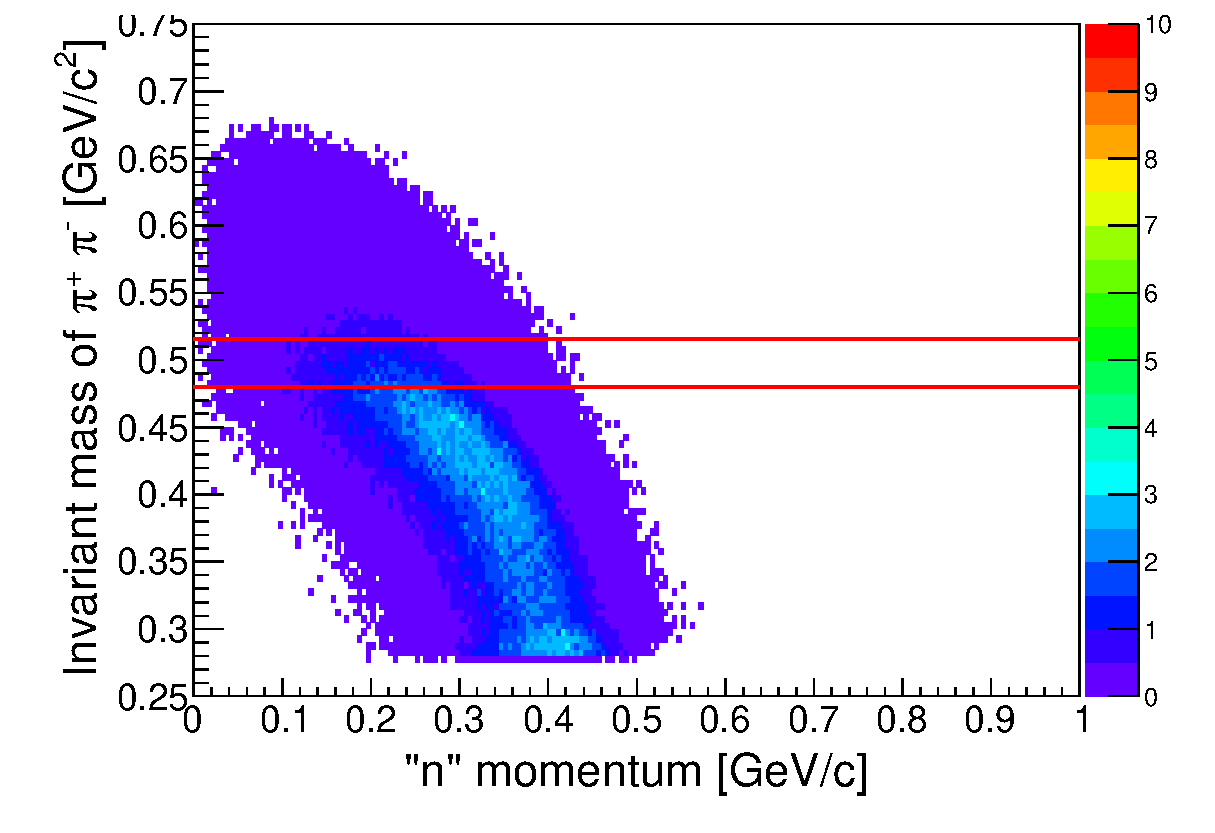
\includegraphics[width=2.5cm]{../pic/Run78/KN_ana/mmN_mom_IM_pipi_pipSm.eps}
      \end{figure}
    }

    \tminipageTwo{
      \begin{figure}
        \tiny
        $K^- d\rightarrow "n" \pi^- \Sigma^+_{forward}$\\
        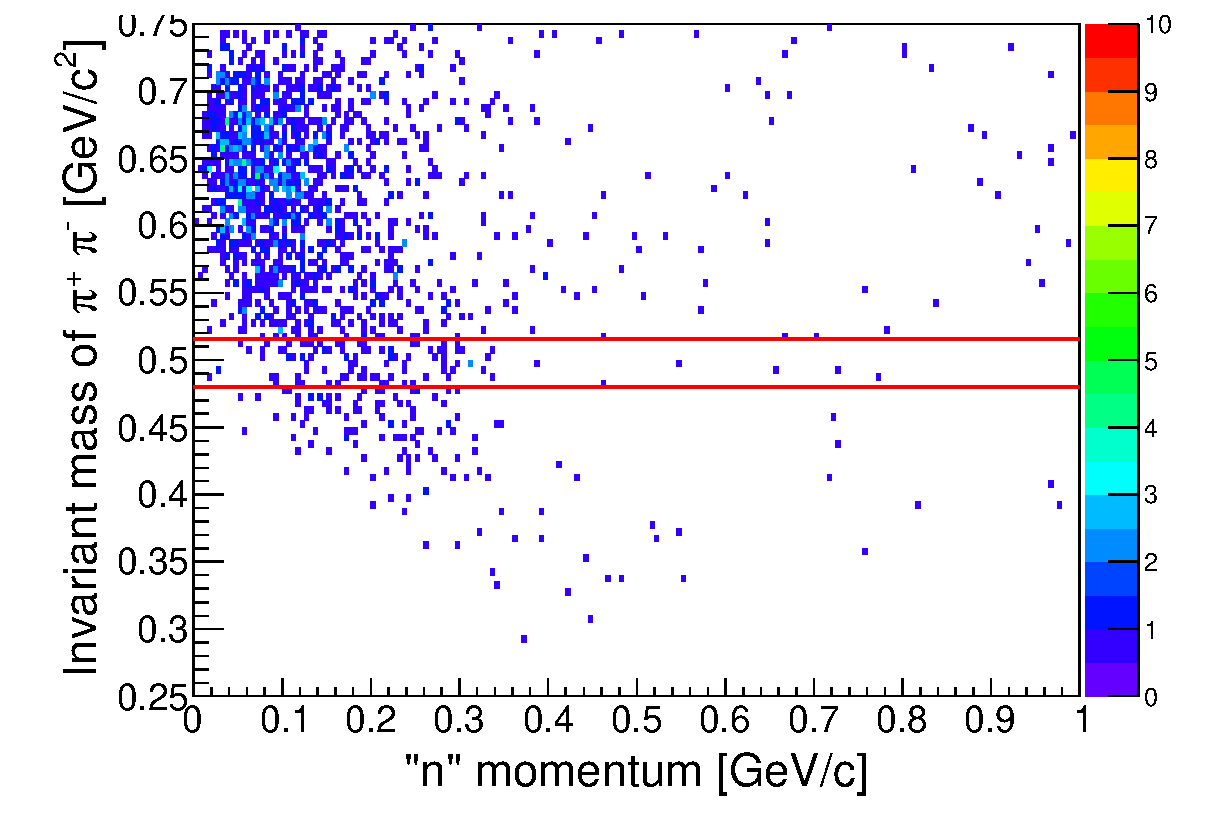
\includegraphics[width=2.5cm]{../pic/Run78/KN_ana/mmN_mom_IM_pipi_Sp.eps}
      \end{figure}
    }{
      \begin{figure}
        \tiny
        $K^- d\rightarrow "n" \pi^+ \Sigma^-_{forward}$\\
        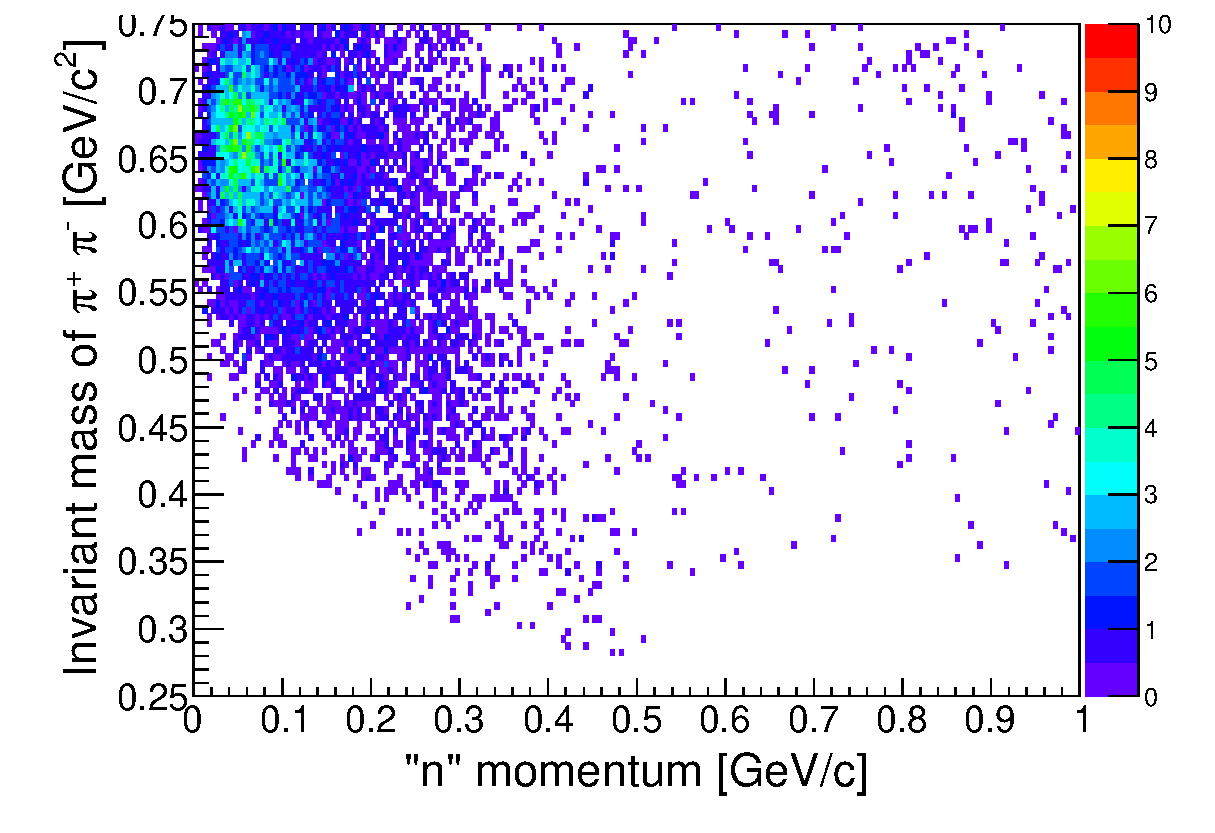
\includegraphics[width=2.5cm]{../pic/Run78/KN_ana/mmN_mom_IM_pipi_Sm.eps}
      \end{figure}
    }
  }
\end{frame}
